\documentclass[crop,tikz]{standalone}                 
\usepackage{physics}
\makeatletter                                                                                        

\begin{document}

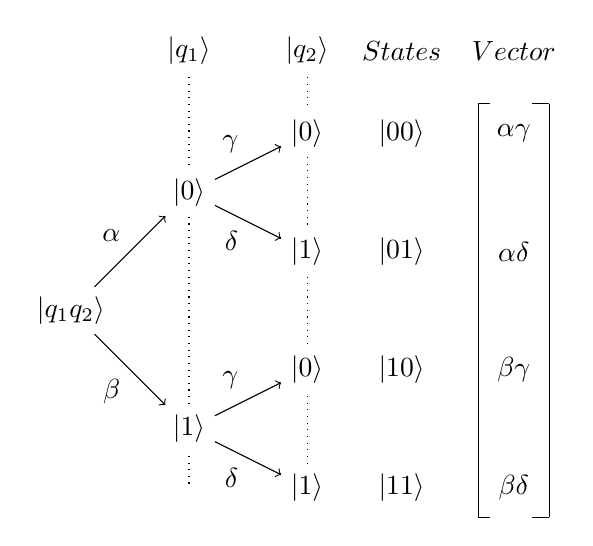
\begin{tikzpicture}[scale=1.5]                                                                          
%\draw [dotted] (0,0) grid (4, 4);

% qubit lines
\draw [-,dotted] ( 1.00, 3.70) -- (1.00,0.00);
\draw [-,dotted] ( 2.00, 3.70) -- (2.00,0.00);
\node [fill=white] (nodeq1) at ( +1.00, +3.70) {$\ket{q_1}$} ;                                           
\node [fill=white] (nodeq2) at ( +2.00, +3.70) {$\ket{q_2}$} ;                                           

% quantum state tree
\node [fill=white]   (nodexx) at ( 0.00, 1.50) {$\ket{q_1q_2}$};                                           
\node [fill=white]   (node0x) at ( 1.00, 2.50) {$\ket{0}$}     ;                                           
\node [fill=white]   (node1x) at ( 1.00, 0.50) {$\ket{1}$}     ;                                           
\node [fill=white]   (node00) at ( 2.00, 3.00) {$\ket{0}$}     ;                                          
\node [fill=white]   (node01) at ( 2.00, 2.00) {$\ket{1}$}     ;                                          
\node [fill=white]   (node10) at ( 2.00, 1.00) {$\ket{0}$}     ;                                          
\node [fill=white]   (node11) at ( 2.00, 0.00) {$\ket{1}$}     ;                                       

\draw [->] (nodexx) -- (node0x) node[midway, above left ] {$\alpha$};
\draw [->] (nodexx) -- (node1x) node[midway, below left ] {$\beta $};                                                           
\draw [->] (node0x) -- (node00) node[midway, above left ] {$\gamma$};                                                           
\draw [->] (node0x) -- (node01) node[midway, below left ] {$\delta$};                                                           
\draw [->] (node1x) -- (node10) node[midway, above left ] {$\gamma$};                                                           
\draw [->] (node1x) -- (node11) node[midway, below left ] {$\delta$};                                                           

% states / configurations
\node [fill=white]   (nodess) at ( 2.80, 3.70) {$States$}  ;                                           
\node [fill=white]   (nodes1) at ( 2.80, 3.00) {$\ket{00}$};                                           
\node [fill=white]   (nodes2) at ( 2.80, 2.00) {$\ket{01}$};                                           
\node [fill=white]   (nodes3) at ( 2.80, 1.00) {$\ket{10}$};                                           
\node [fill=white]   (nodes4) at ( 2.80, 0.00) {$\ket{11}$};                                           

% column vector representation: values
\node [fill=white] (nodevv) at ( +3.75, +3.70) {$Vector$};
\node [fill=white] (nodeaa) at ( +3.75, +3.00) {$\alpha \gamma$};
\node [fill=white] (nodebb) at ( +3.75, +2.00) {$\alpha \delta$};                                          
\node [fill=white] (nodecc) at ( +3.75, +1.00) {$\beta  \gamma$};                                          
\node [fill=white] (nodedd) at ( +3.75, +0.00) {$\beta  \delta$};                                       

% column vector representation: square brackets
\draw [-] ( +3.45, -0.25) -- ( +3.45, +3.25); % right pillar
\draw [-] ( +3.45, -0.25) -- ( +3.55, -0.25); % right cap
\draw [-] ( +3.45, +3.25) -- ( +3.55, +3.25); % right cap
\draw [-] ( +4.05, -0.25) -- ( +4.05, +3.25); % left pillar
\draw [-] ( +4.05, -0.25) -- ( +3.90, -0.25); % left cap
\draw [-] ( +4.05, +3.25) -- ( +3.90, +3.25); % left ca
p
\end{tikzpicture}                                                                                    

\end{document}
